\chapter{Implementation} \label{ch3:implement}

Using the theory provided in the previous chapter the methods are implemented and certain design choices explained. As mentioned in Chapter \ref{ch1:introduction}, software for doing collision detection with \gls{SQ} and \gls{GJK} as well as the \gls{RRT} motion planning algorithm are made. A* is not implemented.

\section{Superquadrics}

Using \gls{SQ} to do collision checking involves using the implicit inside-outside function to check if a specific point lies inside the \gls{SQ} primitive or not. From a memory point of view, one non-deformed \gls{SQ} that has been translated and rotated (collectively referred to \textit{transformed})in space requires eleven parameters to be represented. The transformation operation itself is represented by a $4 \times 4$ matrix (Equation \ref{eq:T}). Note that \gls{SQ} deformations are not implemented.

Since each \gls{SQ} has one $\textbf{T}$ matrix, it is used as the \gls{SQ} state holder in the sense that it contains all of the information necessary to transform the \gls{SQ} from the origin to wherever in space. For plotting purposes, producing the explicit representation using Equation \ref{eq:SQparam} and then doing matrix multiplication with that in accordance with \ref{eq:w->sTransform} will produce points transformed to their designated space. 

Successive transformations can be calculated by $\textbf{T}_{New} = \textbf{T}_n,\dots,\textbf{T}_2\,\textbf{T}_1$ and can from there be assigned as the new state of the \gls{SQ} in question. This is is useful for creating arms composed of \gls{SQ} linked in succession. The new inside-outside function is given by Equation \ref{eq:transformedIOF}, relying on the notation defined in Equation \ref{eq:T_withNotation} for the elements of $\textbf{T}$.

Linking several \gls{SQ} together to form an arm with a base and links (as in Figure \ref{fig:6DoFArm}) is done in the following way:

\begin{enumerate}
	\item Initialize all the \gls{SQ} links and their base in the origin.
	\item For $L_i$ the \textit{i}:th link in the arm (following the base):
	\begin{enumerate}
		\item[2.1] $L_i.\textbf{T} \leftarrow$ $L_{i-1}.\textbf{T}$
		\item[2.2] $L_i.\textbf{T} \leftarrow$ $L_i.Rotate([\phi, \theta, \psi]) \cdot L_i.\textbf{T}$
		\item[2.3] $L_i.\textbf{T} \leftarrow$ $L_i.Translate([p_x, p_y, p_z]) \cdot L_i.\textbf{T}$
	\end{enumerate}
\end{enumerate}

Each link has its transformation matrix as an attribute accessed by "$.\textbf{T}$". Note that the $\cdot$ operation is used here to denote matrix multiplication. Mayavi [\citeauthor{VanderWalt2011}] is used to do the visualizations in this thesis, as seen in Figure \ref{fig:6DoFArm}.

Functions $Translate([p_x, p_y, p_z])$ and $Rotate([\phi, \theta, \psi])$ refer to creating a transformation matrix $\textbf{T}$ that purely translates and purely rotates respectively. In the case of this algorithm specifically, $[\phi, \theta, \psi]$ can be seen as angle commands for the specific joint, and  $[p_x, p_y, p_z]$ is defined as the vector spanning from the top of the previous link to the bottom of the current one (obtained in practice by subtracting the center coordinates of the top and bottom surfaces).

Expressed in words, this algorithm will assign the previous link's transformation matrix to the current one, shifting all the points to where the previous link is located. Then, it will rotate in accordance to outside commands before shifting the current link to connect with the top of the previous link.

\begin{figure}[h]
	\centering
	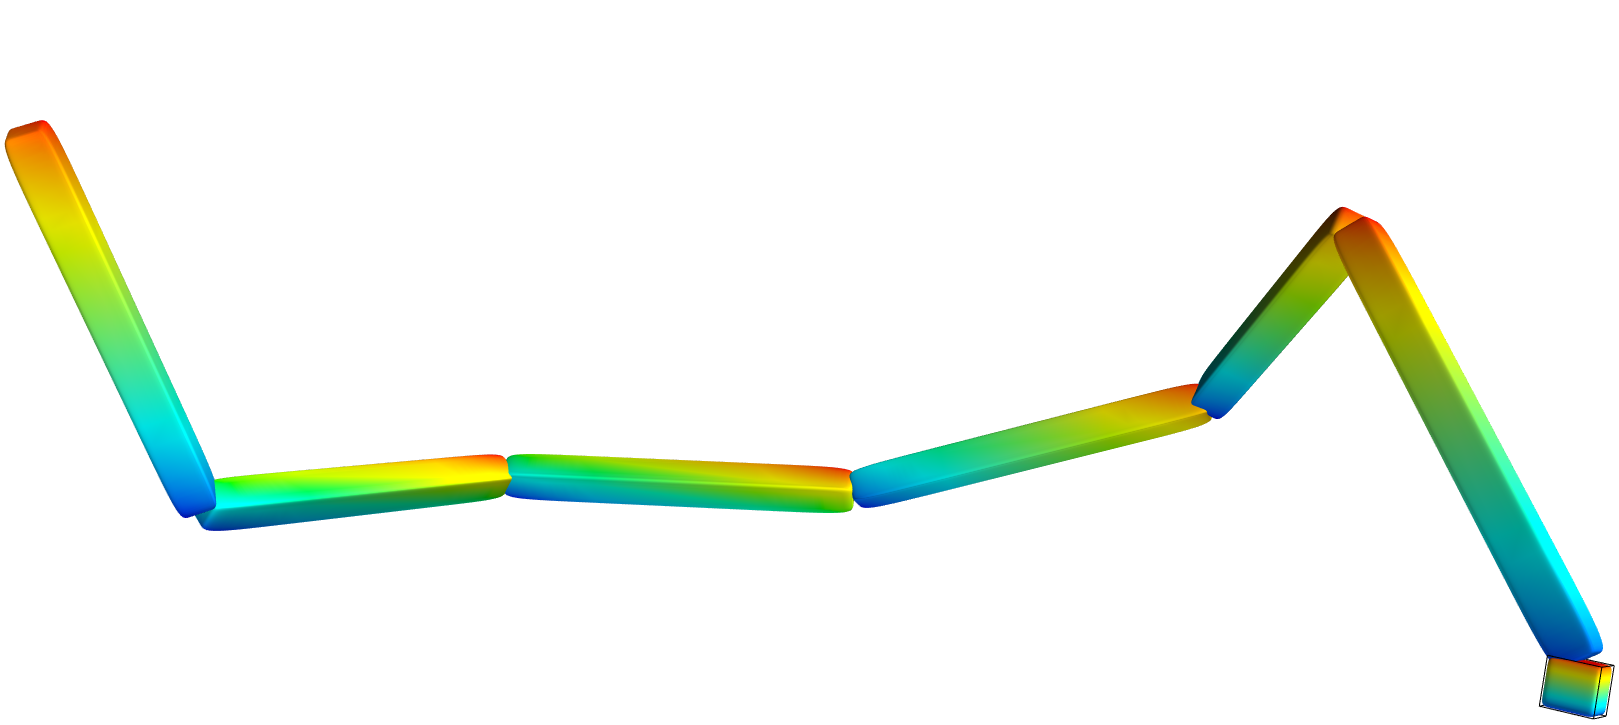
\includegraphics[width=0.7\textwidth]{import/SQ_6DoF_Arm}
	\caption{A seven link arm.}
	\label{fig:6DoFArm}
\end{figure}

\subsection{Intersection Checking} \label{subsec:SQIntersect}

Doing intersection checks with \gls{SQ} requires storing one of the objects implicitly, and the other explicitly. Then, the explicitly stored object has its points looped through the implicit object's inside-outside function, to see if one of them is inside the other object. 

An engineer making use of this method must choose whether the obstacles should be defined explicitly and the robotic manipulator's links implicitly, or if the obstacles should be defined implicitly and the robotic manipulator's links implicitly. The choice will depend on several factors, including how many (relevant) obstacles there are in comparison to the links, which one needs to be perfectly mathematically modeled (i.e. implicitly, to capture a completely accurate) versus which one is okay sample points explicitly, and so on. 

If one class of objects is very large, in order to ensure that the same relative resolution between the obstacles and the links is preserved, a larger number of points will need to be sampled, creating a case for that specific class being implicitly defined. In other words, maintaining $1$ centimeter resolution on a $1 \times 1$ meter grid requires $100^2$ points, and expanding that to a $10 \times 10$ meter grid will result in $1000^2$ points being required to maintain the same resolution. Such an object is better off being represented implicitly, as that only requires $12$ \gls{SQ} parameters and the transformation matrix.

%Simple Binary Search? How does the radial distance come into play+

%making use of simple known SQ translation and rotation, as well as a little about the shape?

\subsection{The Problem of Uniform Angle Sampling} \label{subsec:UniSampleProblem}

%\gls{SQ} can implicitly represent a large number of convex and non-convex shapes, and can through its implicit function very efficiently check point collisions. 
%
%On the other hand, however, e
%
Explicitly representing the \gls{SQ} by naively producing points through uniform sampling points of the angles $\eta$ and $\omega$ might result in some unwanted behavior. 

Producing the coordinates in accordance with Equation \ref{eq:SQparam} by uniformly sampling the angles (from $\frac{-\pi}{2}$ to $\frac{\pi}{2}$ and from  $-\pi$ to $\pi$ respectively) will not necessarily result in uniformly spread points in the real world, especially for $\epsilon$-values below 1. This issue was discovered while testing the collision detection method for a four link arm, as shown in Figure \ref{fig:SQ_UniSampling}. 

\begin{figure}[h]
	\centering
	\begin{minipage}[h]{0.3\textwidth}
		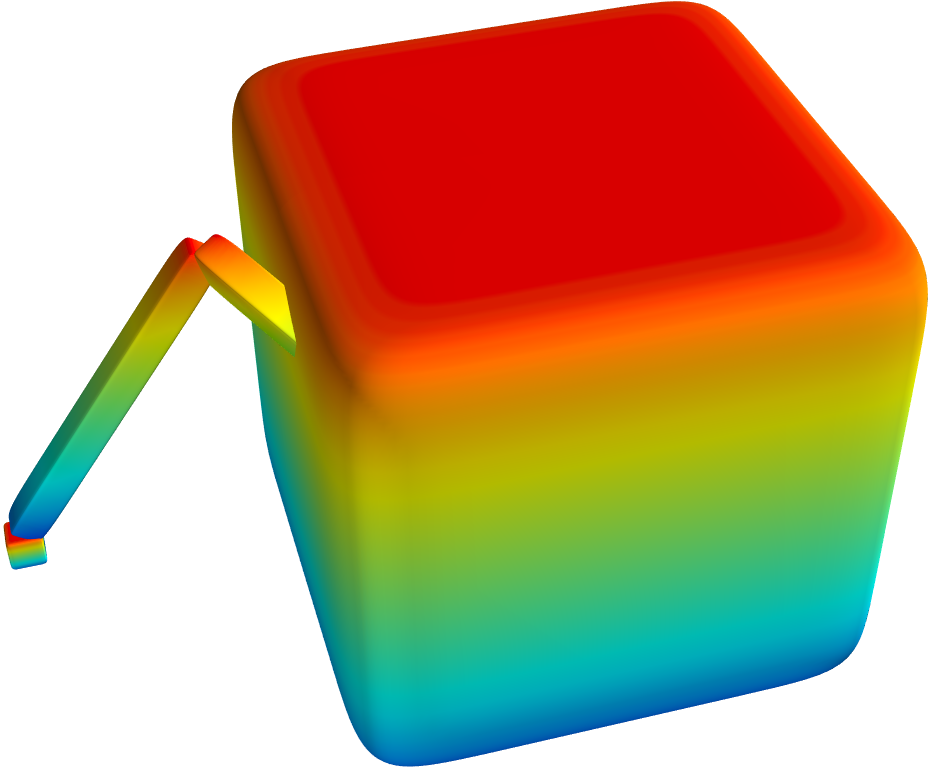
\includegraphics[width=1\textwidth]{import/SQ_ObsBox_Collision}
		\subcaption{Box-shaped ($\epsilon_1=\epsilon_2=0.2$) SQ obstacle. The algorithm failed to register the collision.}
		\label{fig:SQ_ObsBoxCol}
	\end{minipage}
	\hspace{1cm}
	\begin{minipage}[h]{0.3\textwidth}
		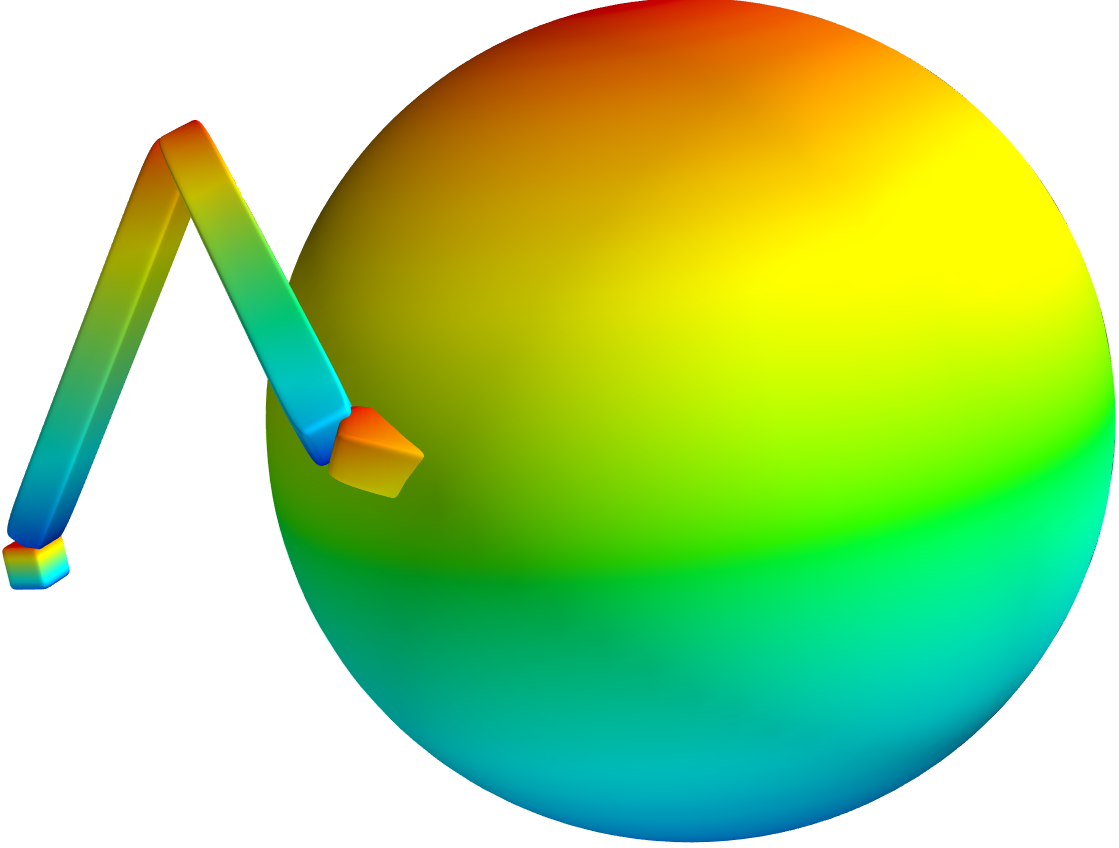
\includegraphics[width=1\textwidth]{import/SQ_ObsSphere_Collision}
		\subcaption{Spherical  ($\epsilon_1=\epsilon_2=1$) SQ obstacle. The algorithm correctly registered collision. }
		\label{fig:ObsSphCol}
	\end{minipage}
	\caption{Collision detection testing with a three link arm.}
	\label{fig:SQ_UniSampling}
\end{figure}

In the case of the box-shaped obstacle (shown in Figure \ref{fig:SQ_ObsBoxCol}), due to the non-uniform spread of the points, the algorithm did not detect the collision. This problem can be clearly understood by going down to two dimensions and plotting superellipses (refer to Equation \ref{eq:SuperEllipse}), as seen in Figure \ref{fig:Superellipses}.

\begin{figure}[h!]
	\centering
	\begin{minipage}[h]{0.7\textwidth}
		\centering
		\subcaption{Square-shaped superellipse. Note the conspicuous lack of points along the sides.}
		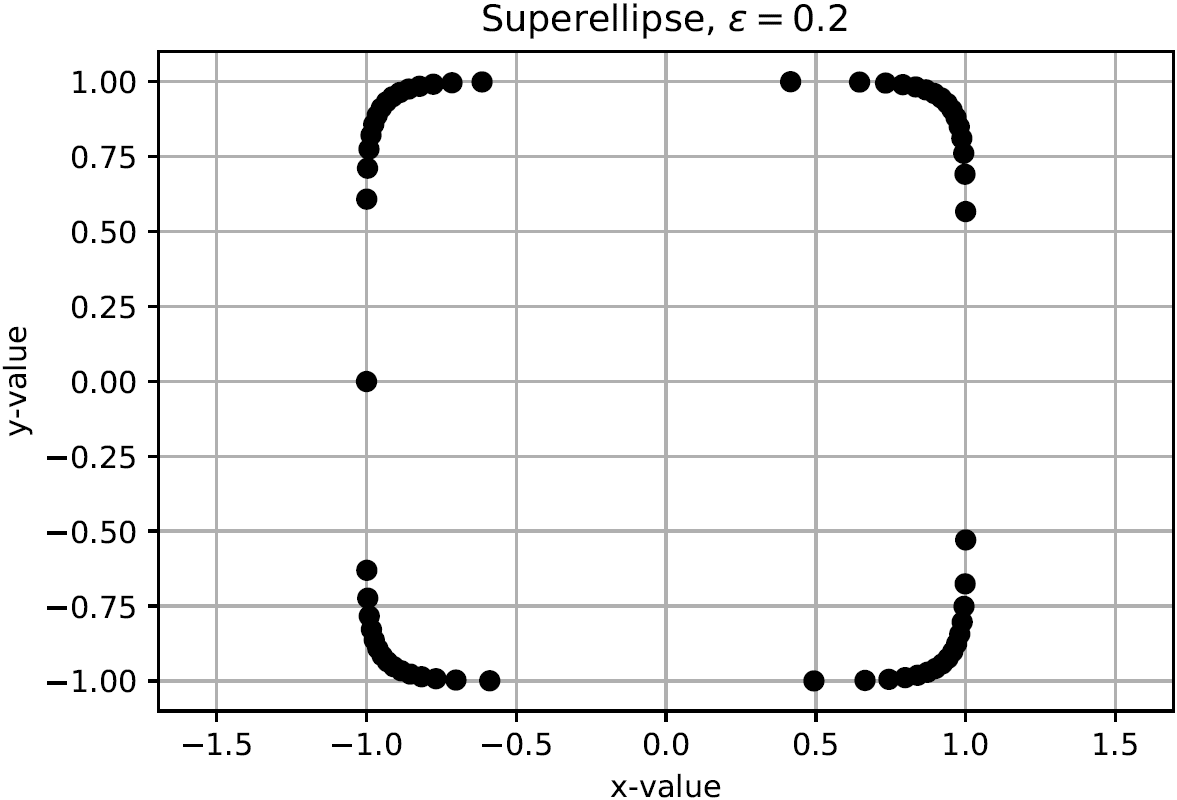
\includegraphics[width=1\textwidth]{import/Se_Square}
		\label{fig:Se_Square}
	\end{minipage}
	%	\hspace{1cm}
	\begin{minipage}[h]{0.3\textwidth}
		\subcaption{Circle-shaped superellipse.}
		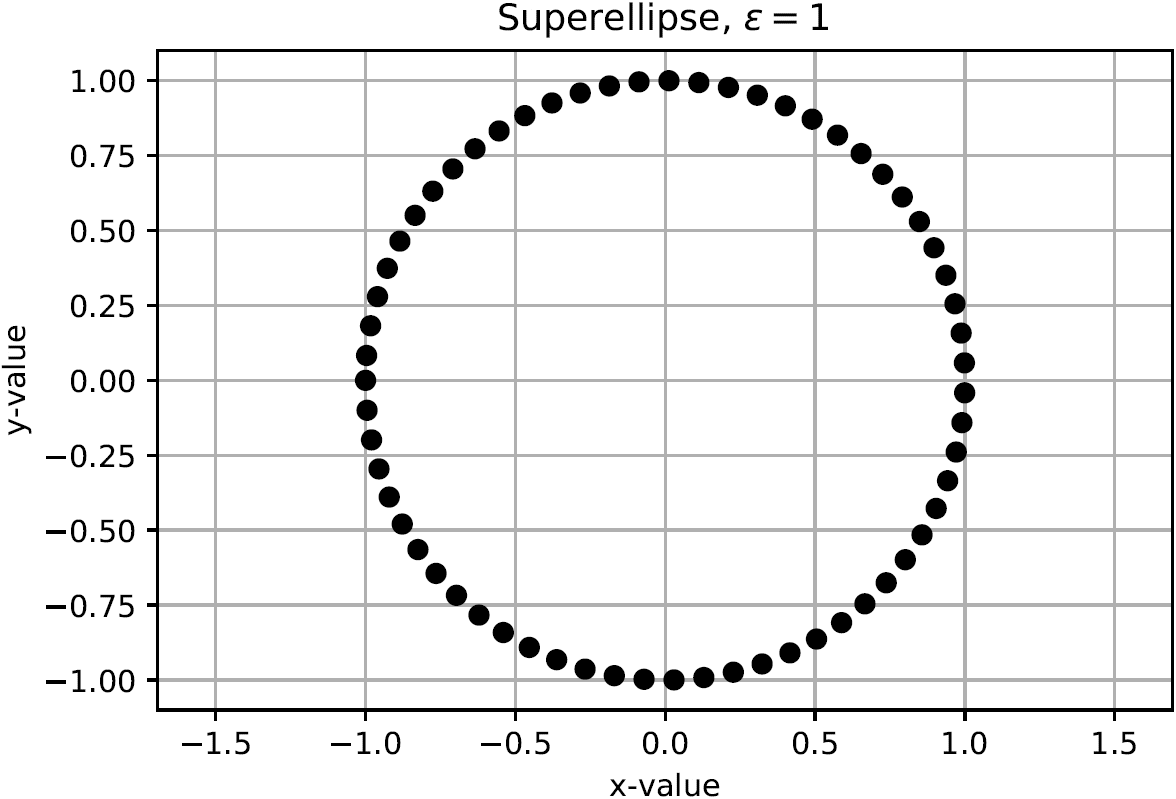
\includegraphics[width=1\textwidth]{import/Se_Round}
		\label{fig:Se_Circle}
	\end{minipage}
	%	\vspace{2 cm}
	\begin{minipage}[h]{0.3\textwidth}
		\subcaption{Rhomb-shaped superellipse.}
		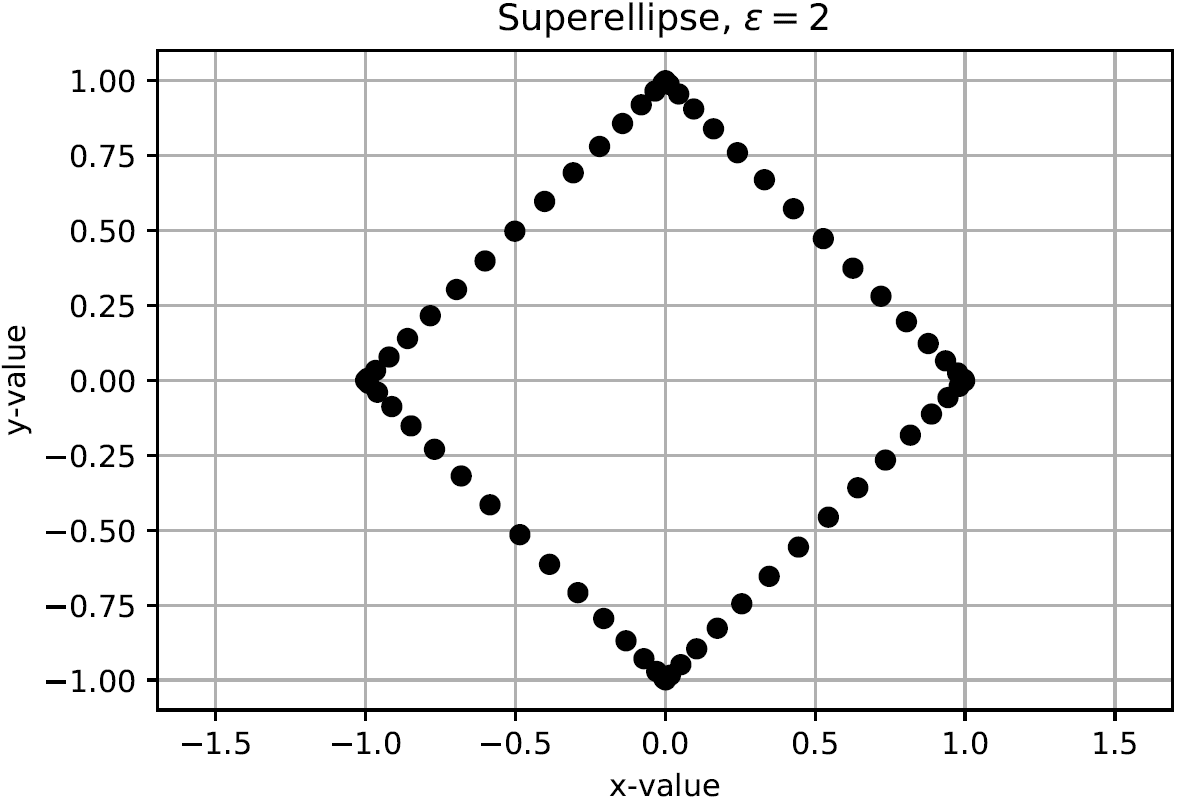
\includegraphics[width=1\textwidth]{import/Se_Rhomb}
		\label{fig:Se_Rhomb}
	\end{minipage}
	%	\hspace{1cm}
	\begin{minipage}[h]{0.3\textwidth}
		\subcaption{Concave-shaped superellipse.}
		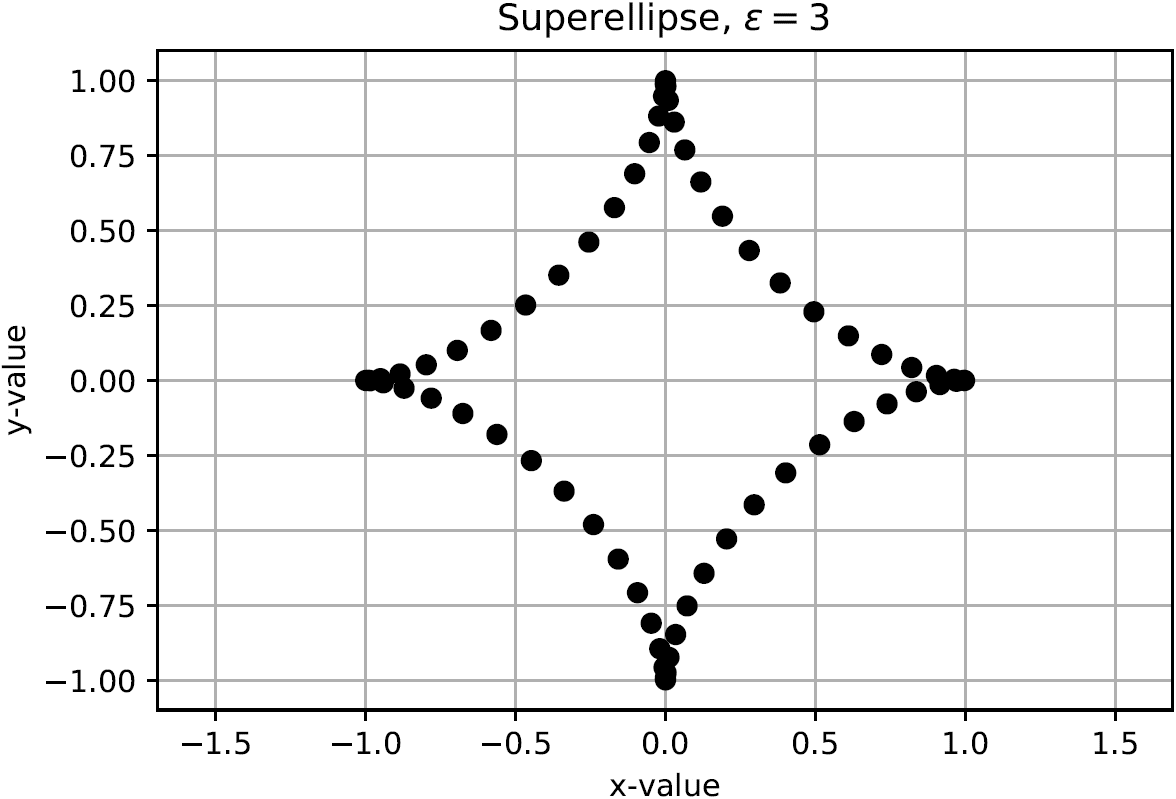
\includegraphics[width=1\textwidth]{import/Se_Concave}
		\label{fig:Se_Concave}
	\end{minipage}
	\caption{Four different superellipses sampled from $-\pi$ to $\pi$ with the same increment value.}
	\label{fig:Superellipses}
\end{figure}

For larger $\epsilon$ values the points are spread quite uniformly, but for values below 1 the points are concentrated along the corners. Thus, for this method to effectively work with box-shaped obstacles specifically, the points cannot be uniformly sampled over the angle values. It can either be improved with selective sampling, or simply replaced with a grids of points oriented to resemble a box in accordance with the $a_1, a_2$ and $a_3$ values defining the lengths of the sides. Naturally, this is not an issue when implicitly representing box-shaped objects..

Note that while it would be possible to rotate a rhomb-shaped superellipse (Figure \ref{fig:Se_Rhomb}) to get a square shape, simply setting $\epsilon_1=\epsilon_2=2$ results in a double-pyramid shaped \gls{SQ} and not a rotated cube.

Also, note that the reverse of this problem is encountered for very large $\epsilon$ values. Such superellipses resemble crosses (or increasingly pinched versions of Figure \ref{fig:Se_Concave}), whose points become more and more concentrated in the center.


\section{GJK}
As first mentioned in Section \ref{subsubsec:GJKiter}, the implementation of \gls{GJK} used in this thesis relies on a geometric approach that makes use of vector algebra. The \textit{n}-simplex $\mathcal{W}$ only goes between five different stages:

\begin{enumerate}
	\item[$-$] $0$-simplex: The empty set, before the algorithm starts.
	\item[$-$] $1$-simplex: The set is a point in $K_C$.
	\item[$-$] $2$-simplex: The set is a line between two points.
	\item[$-$] $3$-simplex: The set is a triangle, as seen earlier in Figure \ref{fig:GJK_E}.
	\item[$-$] $4$-simplex: The set is a pyramid, as can be seen in Figure \ref{fig:GJK_CBA}. The algorithm tries to encapsulate the origin.
\end{enumerate}

The algorithm does not go beyond that. If $K_C$ surrounds the origin (i.e., $K_A$ and $K_B$ are in collision) a $4$-simplex encapsulating it will eventually be able to be set up.

A $4$-simplex is composed of four sides of $3$-simplices. By keeping track of which order the points were added to the simplex, as well as using vector algebra (dot and cross products specifically), simple operations such as checking which point, edge, or face is facing towards the origin can be performed.

As an example, consider the $2$-simplex case. Using the same notation as in Figure \ref{fig:GJK_E}, the simplex is composed of $\mathcal{W} = \{B,A\}$, where $B$ was added previously and $A$ in the current iteration. The algorithm is trying to answer the following: is the origin closest to $A$, $B$, or the line $AB$? 

\begin{enumerate}
	\item[$AB$] Check this case first. If the origin is in the $AB$ Voronoi region defined as all the points closest to the line $AB$ (i.e. $AB\,\cdot \,(-A)\,>0$), both $A$ and $B$ should be kept and the next search direction will be in the direction perpendicular to $AB$ in the direction of the origin. This new direction can be calculated using a double cross-product: $AB\, \times \,(-A)\,\times\, AB$.
	\item[$A$] Check this case after having checked the previous one. If the origin is closest to $A$, $B$ can be discarded and a new point in the extreme direction of $-A$ can be added to the simplex.  A new point will be produced and checked to see whether it is on $A$'s side of the origin, or if it is actually beyond the origin. In the latter case the new point will be added to the simplex as the new $A$ while the old $A$ becomes the new $B$.
	\item[$B$] This case is not checked because it is assumed to be impossible because of the way the algorithm will have produced $A$. $A$ was produced in the direction of the origin, such that either a point on the line $AB$ will be closer to the origin, or that point is $A$ itself. 
\end{enumerate}
%In fact, I think according to the most recent optimization

This geometric approach can be extended to $3$-simplices, where $\mathcal{W} = \{C, B, A\}$. The same kind of optimization could also be applied, where there is no point in checking $C$, $B$ or the edge $BC$ because they should have been already checked as part of getting to the current $A$. Depending on whether the origin is closest to $AC$, $AB$ or the new $A$ region points are expelled and directions set.

For $4$-simplices, each face, with the exception of the now previously visited $DCB$ triangle, is checked individually to see if the point is either "below" the plane defined by the triangle (i.e. towards the inside of the pyramid $4$-simplex) or anywhere else. As this is a binary response, eight different ($2^3$) scenarios are considered and measures are taken depending on each of them.

%For more information, refer to the \gls{GJK} collision detection code.


\subsection{Support Mapping Function}

A general support function is used, not one particularly optimized to a specific shape. As a function, it is applied once on $K_A$ and once on $K_B$ with the search direction reversed in the latter case, with the result for $K_C$ obtained by subtracting them.

The following Python code takes a list of Numpy array \textit{points} and a Numpy array \textit{direction}, as well as a \textit{reverse} boolean to reverse the direction when using this function for $K_B$. 

It will loop through all the points in \textit{points} and finds the one that is most extreme in the \textit{direction} by taking their dot product and comparing the result with previous dot products. The most extreme will produce the biggest dot product. Numpy is a scientific computing package for Python ([\citeauthor{TravisE2006}], [\citeauthor{VanderWalt2011}]).

\begin{lstlisting}
def support_mapping_function(points, direction, reverse=False):
	if reverse==True: 
		direction = -1*direction
	bestIndex = 0
	bestDotP = numpy.dot((points[0][bestIndex], points[1][bestIndex], points[2][bestIndex]), direction)
	for i in range(len(points)):
		dotProd = numpy.dot([points[0][i], points[1][i], points[2][i]], direction)
		if dotProd>bestDotP:
		bestIndex = i
		bestDotP = d
	furthestPoint = numpy.array([points[0][bestIndex], points[1][bestIndex], points[2][bestIndex]])
	return furthestPoint
\end{lstlisting}



\subsection{Termination Conditions}

The algorithm will return either \textit{True} (collision) or \textit{False} (no collision), but there are four overall different ways for it to terminate into these. Note that unlike the general algorithm in \ref{subsubsec:GJKiter}, the one implemented for this thesis does not care about the specific distance between the object, just whether or not they intersect.

The following cases will result in the algorithm terminating:

\begin{enumerate}
	\item[$-$] Termination Condition 1: If when generating a new point $\textbf{w}_{i+1}$ in some direction $\textbf{-v}$ the new point is not on the other side of the origin, it means that all points of $K_C$ exist on the $\textbf{+v}$ side of the origin and thus the origin is not surrounded by $K_C$. Thus, we can conclude that there is no collision. See Figure \ref{fig:GJK_TC1} for an example.
	\item[$-$] Termination Condition 2: If the new support point $\textbf{w}_{i+1}$ is arbitrarily close to the origin we can assume that a collision took place. In practice, the algorithm checks $abs(\textbf{w}_{i+1}) < \textbf{e}_{tol}$, where $\textbf{e}_{tol}$ is set to something arbitrarily small like $\textbf{e}_{tol} = (0.1, 0.1, 0.1)^T$. 
	\item[$-$] Termination Condition 3: If the algorithm can construct a $4$-simplex (pyramid) that encapsulates the origin, the origin is obviously part of $K_C$ and a collision happened.
	\item[$-$] Termination Condition 4: If the algorithm is stuck in a loop of creating and dismissing various constellations of simplices, it can be assumed that a collision occurred. The variable $i_{max}$ is used to define an upper limit on the allowed algorithm iteration loops. 
\end{enumerate}


\begin{figure}[h]
	\centering
	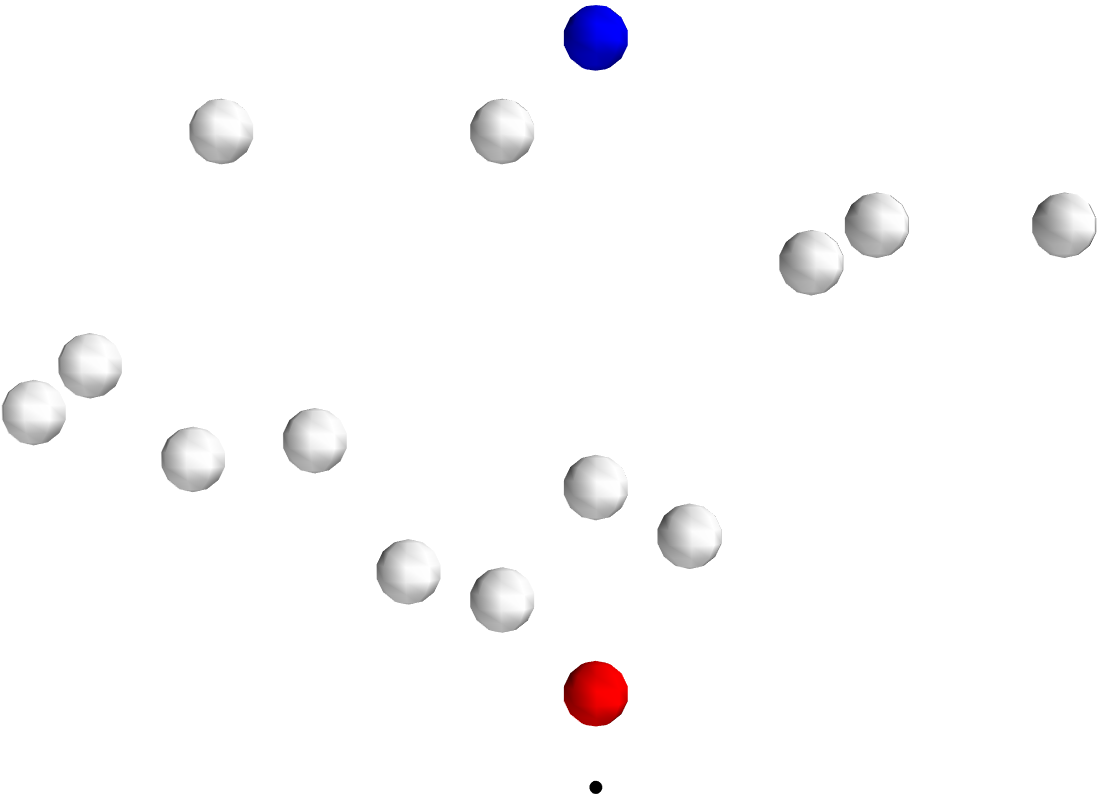
\includegraphics[width=0.5\textwidth]{import/GJK_TC1}
	\caption{The set of points (in the $x$-$y$-plane) are all to one side of the origin (Black). Blue $(0,0, 10)^T$ was arbitrarily chosen in the initial steps and Red $(0,0,1)^T$ is the point most extreme in direction $(0, 0, -10)^T$. The algorithm terminates according to Termination Condition 1. Note that the points are inflated for visual purposes only.}
	\label{fig:GJK_TC1}
\end{figure}

The algorithm is sensitive to two things. The first is the explicit representation of the object: how many points where used to define $K_A$ and $K_B$ (i.e., the link and the obstacle)? More points is more accurate, but worse in terms of memory and the computation time for the support mapping function. The second factor it is sensitive to is numerical precision.

\begin{figure}[h]
	\centering
	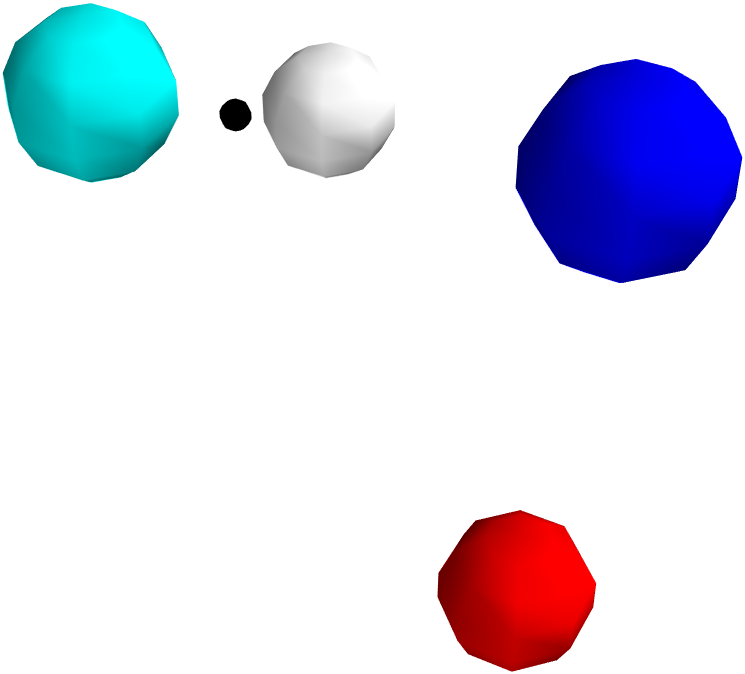
\includegraphics[width=0.3\textwidth]{import/GJK_CBA_triangle}
	\caption{A $4$ simplex (White-Blue-Cyan-Red) with the origin (Black). Note that the points have been inflated for visual purposes only. Also, note that the origin was purposefully rendered to be much smaller than the other four points, which are different in size due to the perspective.}
	\label{fig:GJK_CBA}
\end{figure}

Termination Condition 4 might at first glance look like a very weak condition by itself, but it is acceptable because Termination Condition 1 is so strong that if the algorithm does get stuck in a loop it can be assumed that it is due to the aforementioned factors. For example, in Figure \ref{fig:GJK_CBA} the origin is actually (if barely) inside the $4$-simplex. But due to numerical imprecision, the algorithm misses this and does not register the Blue-Cyan-White triangle $3$-simplex as being above it. Thus, the algorithm iterates $i_{max}$ times until it is forcefully terminated.

It is worth pointing out that in the example that produced Figure \ref{fig:GJK_CBA}, $K_A$ and $K_B$ were two spheres with radius $1$ length units represented by $20^2$ points each. $K_B$ had been translated $2.01$ length units in the $x$-axis. When translated $2.02$ length units, the algorithm terminated in accordance with the Termination Condition 1.


\section{RRT}

The \gls{RRT} algorithm is implemented as listed in Section \ref{subsubsec:RRRTAlgo}. To generate distance, it uses the Euclidean distance between the angles in C-space. When generating $\textbf{p}_{random}$, at a specific count (e.g., every 100th sampled point) it will return the goal configuration instead of a randomly sampled point in order to help it converge faster and not have it blindly explore the whole C-space.

Though a goal configuration exists and is used for the biasing, in practice the aim is to have the tip of the robotic manipulator (typically, the \gls{EE}) within a goal region. Thus, in this implementation, the algorithm terminates once the tip of the final link has entered a specific goal region. Whether or not the whole robotic manipulator is in the exact same angle configuration or pose as the goal configuration is not as relevant.

The two collision detection methods can be used interchangeably. The functions receive a specific arm configuration, check if it collides with the obstacles of the world and returns a boolean. When checking a line segment, if a collision is found the algorithm discards the point completely. %Note that no self-collision check has been implemented.

\section{Simulation Design and Measurements}

In accordance with \textbf{RQ1a} and what was stated in the Methodology section of Chapter \ref{ch1:introduction}, the \gls{SQ} and \gls{GJK} algorithms will be tested with each other. As they are used as black box methods in the \gls{RRT} algorithm, it makes sense to test them separately with each other as the \gls{RRT} should simply act as a multiplicative factor that is the same for both algorithm. Nevertheless, the full \gls{RRT}+\gls{SQ} and \gls{RRT}+\gls{GJK} algorithms will be tested for the sake of clarity.

Note that both algorithms will use objects generated by the \gls{SQ} class implemented. The \gls{SQ} class can generate convex shapes ($\epsilon_1 \leq 2$ and $\epsilon_2 \leq 2$) and store them explicitly, so it is useful for generating the links and obstacles that the \gls{GJK} can take. For each \gls{SQ} object, the points will be generated over $\eta$ and $\omega$, from $-\pi/2$ to $\pi/2$ and from $-\pi$ to $\pi$ respectively. The amount of points generated in these intervals is determined by the parameter $n$, which sets the increment size. Thus, due to the spherical product, each \gls{SQ} has $n^2$ number of points.

The following factors are deemed to have an effect on the collision detection computation time of the algorithms:
\begin{enumerate}
	\item Number of links $l$.
	\item Number of obstacles $o$.
	\item \gls{SQ} increment parameter $n$.
	\item \gls{GJK}'s max iteration threshold $i_{max}$.
	\item Convexity: \gls{GJK} only works for convex shapes.
\end{enumerate}

When testing how the algorithms perform relative each other, it is of interest to set up experiments that examine how the algorithms compare with each other when the aforementioned parameters (sans the convexity clause) are varied. 
